\documentclass[hyperref={bookmarks=false},aspectratio=169]{beamer}
\usepackage[utf8]{inputenc}
\usepackage{standalone}
% ---------------  Define theme and color scheme  -----------------
\usetheme[sidebarleft]{CEIT}  % 3 options: minimal, sidebarleft, sidebarright
\usepackage{fontspec}
\newfontfamily{\ps} [ Path = ./fonts/]{TypeWheel-Regular.ttf}

%\setbeamertemplate{footline}[frame number]
\setbeamertemplate{footline}[text line]{%
	\parbox{\linewidth}{\vspace*{-8pt} \textcopyright \  Centre for Development of Advanced Computing (C-DAC)  \hfill \insertpagenumber}}
\setbeamertemplate{navigation symbols}{}

\usepackage{ragged2e}


% ------------  Information on the title page  --------------------
\title[PPT Title]
{\bfseries{Database Concepts}}

\subtitle{Lab Session 1}

\author[Jishnu T U] %\& Managed]
{Jishnu T U\inst{1} } %\and Managed\inst{2}}

\institute[CEIT]
{
  \inst{1}
  Trainer\\
  Centre of Excellence in IT,PNG
 % \and
 % \inst{2}
 % Trainer\\
 % Centre of Excellence in IT,PNG
}

\date[CEIT, 2014]
{Centre of Excellence in IT,PNG October 2019}
%------------------------------------------------------------

%------------------------------------------------------------
%The next block of commands puts the table of contents at the 
%beginning of each section and highlights the current section:

\AtBeginSection[]
{
  \begin{frame}
    \frametitle{Table of Contents}
    \tableofcontents[currentsection]
  \end{frame}
}

%------------------------------------------------------------


\begin{document}

\frame{\titlepage}  % Creates title page

%---------   table of contents after title page  ------------
\begin{frame}
\frametitle{Table of Contents}
\tableofcontents
\end{frame}
%---------------------------------------------------------


%\section{Introduction to Oracle}
\begin{frame}

	\frametitle{ Introduction to Oracle}
	
	\begin{itemize}
	
	    \item
	
	    \item
	
	\end{itemize}

\end{frame}
\begin{frame}

	\frametitle{MS SQL Server}
	
	\begin{itemize}
	
	    \item SQL Server is a relational database management system (RDBMS) developed and marketed by Microsoft.
	
	    \item  As a database server, the primary function of the SQL Server is to store and retrieve data used by other applications.
	
     	\item  SQL Server is built on top of SQL, a standard programming language for interacting with the relational databases. 
     	
     	\item SQL server is tied to Transact-SQL, or T-SQL, the Microsoft’s implementation of SQL that adds a set of proprietary programming constructs
     	
     	\item SQL Server consists of two main components:
     			\begin{enumerate}
     		
     		\item 	Database Engine
     		
     		\item 	SQLOS 
     		
     	\end{enumerate}
     
     
     	
	
	\end{itemize}
	
\end{frame}


\begin{frame}
	
	\frametitle{MS SQL Architecture}
	
	\begin{figure}
		\centering
		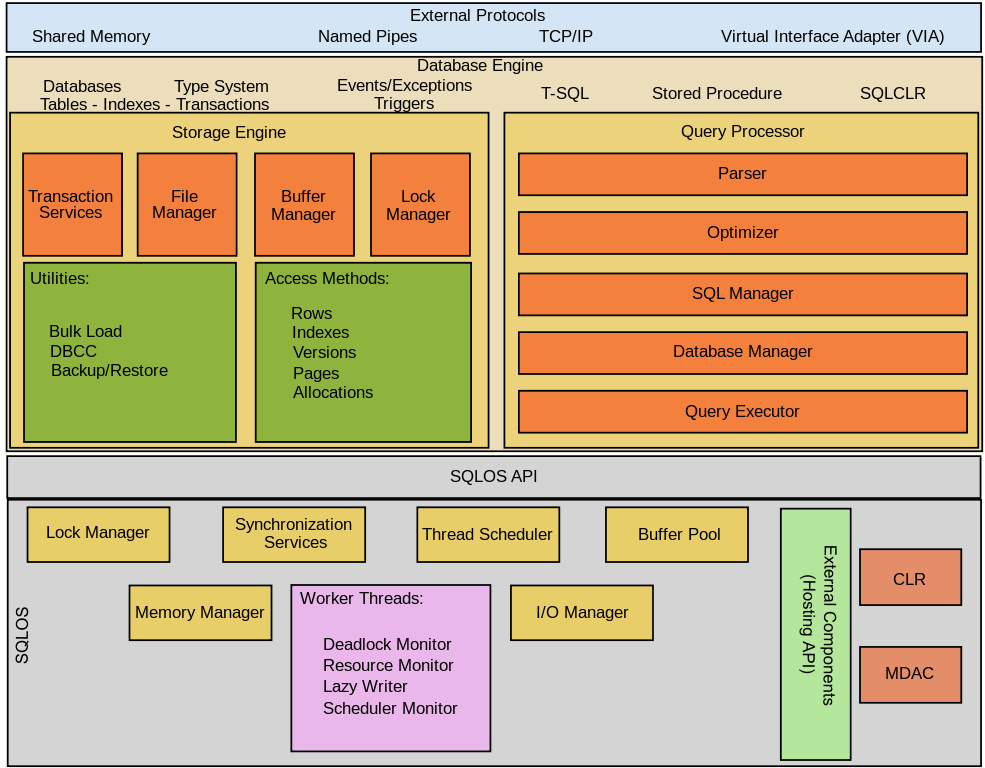
\includegraphics[width=300pt,height=210pt]{figures/What-is-SQL-Server-SQL-Server-Architecture.png}
	\label{fig:ms sql architecture}
\end{figure}

\end{frame}


\begin{frame}
	\frametitle{MS SQL Architecture}
	
	\begin{columns}
		
		\column{0.45\textwidth}
		
\textbf{Database Engine:}  The Database Engine consists of a relational engine that processes queries and a storage engine that manages database files, pages, pages, index, etc
The database objects such as stored procedures, views, and triggers are also created and executed by the Database Engine.

\textbf{SQLOS} : SQLOS provides many operating system services such as memory and I/O management. Other services include exception handling and synchronization services.
	


		
		
		\column{0.55\textwidth}

		
		\textbf{Relational Engine} : The Relational Engine(query processor) contains the components that determine the best way to execute a query.
		
		The relational engine requests data from the storage engine based on the input query and processed the results.
		
		Some tasks of the relational engine include querying processing, memory management, thread and task management, buffer management, and distributed query processing.
		
		\textbf{Storage Engine} : The storage engine is in charge of storage and retrieval of data from the storage systems such as disks and SAN.
					
	\end{columns}
\end{frame}

\begin{frame}
	
	\frametitle{Microsoft SQL Server Management Studio}
	
	\begin{itemize}
		
		\item To interact with SQL Servers, you need to install SQL Server Management Studio (SSMS).
		
		\item  The SQL Server Management Studio is a software for querying, designing, and managing SQL Server on your local computer or in the cloud. 
		
		\item It provides you with tools to configure, monitor, and administer SQL Server instances.
		
	\end{itemize}
	
\end{frame}



\begin{frame}
	
	\frametitle{Microsoft SQL Server Management Studio}
		
		Let's start practicing...
		 
	\input{lab_pgm/version.sql}

\end{frame}
\begin{frame}
\frametitle{}
\begin{figure}
    \centering
    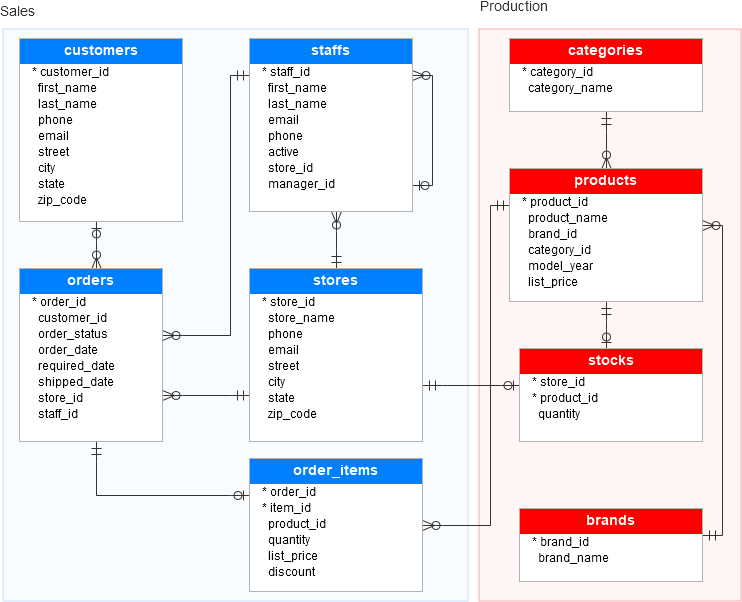
\includegraphics[width=300pt,height=210pt]{figures/SQL-Server-Sample-Database.png}\end{figure}
\end{frame}

\begin{frame}
	\frametitle{ DB and Schema}
	
	\begin{itemize}
	
	    \item<1->  \textbf{Activity :}
	    
	     Create database 'university\_db' and schema 'university' for the  
	
	    \item<2->   
	    {\ps
	    	
	    	
	    	     	
	    	
	    }
	
	\end{itemize}
	
\end{frame}

\section{ SQL* Plus}

\begin{frame}

	\frametitle{ SQL* Plus}
	
	\begin{itemize}
	
	    \item
	
	    \item
	
	\end{itemize}
	
\end{frame}
\section{ DDL Commands}

\begin{frame}
	\frametitle{ DDL Commands}
	
	\begin{itemize}
	
	    \item
	
	    \item
	
	\end{itemize}
	
\end{frame}
\begin{frame}
	\frametitle{ DDL Commands}
	
	\begin{itemize}
	
	    \item<1->  \textbf{Problem :}
	    
	     Create a table 'students' with columns student\_id, first\_name, last\_name, email\_id, dob ?
	
	    \item<2->   
	    {\ps
	    	
	    	
	    	 CREATE TABLE students 
	    	
	    	(student\_id INTEGER AUTO\_INCREMENT PRIMARY KEY, 
	    	
	    	first\_name VARCHAR(50), 
	    	
	    	last\_name VARCHAR(50), 
	    	
	    	email\_id VARCHAR(255),  
	    	
	    	dob DATE);
	    	
	    	
	    }
	
	\end{itemize}
	
\end{frame}
\section{DML  Commands}
\begin{frame}

	\frametitle{ DML  Commands}
	
	\begin{itemize}
	
	    \item
	
	    \item
	
	\end{itemize}
	
\end{frame}
\section{ DCL Commands}
\begin{frame}

	\frametitle{  DCL Commands}
	
	\begin{itemize}
	
	    \item
	
	    \item
	
	\end{itemize}
	
\end{frame}

\end{document}